\documentclass[11pt,notitlepage]{article}

\usepackage[comma,numbers,sort&compress]{natbib}
\usepackage{graphicx}
\usepackage{color}
\usepackage{soul}
\usepackage{amssymb}
\usepackage{amsbsy}
\usepackage{theorem}
\usepackage{xcolor}
\usepackage{fullpage}
\usepackage{amsmath}
\usepackage{bm}
\usepackage{empheq}
\usepackage{centernot}
\usepackage{mathtools}
\usepackage{stmaryrd}
\usepackage[margin=1cm,skip=2pt]{caption}
\usepackage{algorithmic}
\usepackage{helvet}
\renewcommand{\familydefault}{\sfdefault}
\usepackage[affil-it]{authblk}
\usepackage[margin=1in]{geometry}
\usepackage{caption}
\usepackage{hyperref}
\captionsetup{font=small}
\usepackage[percent]{overpic}     % allows for plot annotations like subplot panel labels

\usepackage{titlesec}

\titlespacing\section{0pt}{12pt plus 4pt minus 2pt}{0pt plus 2pt minus 2pt}
\titlespacing\subsection{0pt}{12pt plus 4pt minus 2pt}{0pt plus 2pt minus 2pt}
\titlespacing\subsubsection{0pt}{12pt plus 4pt minus 2pt}{0pt plus 2pt minus 2pt}
\setlength{\parindent}{0cm}


\begin{document}

\thispagestyle{plain}
\pagenumbering{gobble}

\section{Summary vision statement}
\setlength{\parskip}{4pt} Our proposal describes a knowledge engine in the
spirit of Wolfram$|$Alpha \cite{Wolframalpha}: the user will query the system in
natural language and the knowledge engine will parse the input, generate search
strategies to fulfill the user question, execute user-selected search strategies
by traversing the relevant Knowledge Sources, and finally present results to the
user. Similar to the highly successful Wolfram$|$Alpha, our knowledge engine
will learn from repeated interactions with users to return the most relevant
search strategies for a given type of natural language query.

This system will handle a variety of user queries spanning the spectrum of
biomedical entity types in available Knowledge Sources. In
%by the content and variety of the NCATS Translator knowledge beacons. In
particular, our proposed solution will be able to process queries involving a
number of biological entities, with example questions including: \textit{How are
  disease X and Y related?}, \textit{How does variant X cause disease Y and
  protect against disease Z?}, \textit{What is the clinical outcome pathway for
  the treatment of disease X by drug Y?}, \textit{For all drugs used to treat
  disease X, which ones have the least well-studied clinical outcome pathway?},
etc.

Our approach (detailed in the project description) would advance current
capabilities for biomedical knowledge querying in several respects. First, the
process of generating and executing search strategies will be automated,
removing the need to write custom Python notebooks for each query type. Our
system, based on a probabilistic Markovian architecture, will both learn from
repeated user interaction and also dynamically incorporate uncertainty in all
steps of the proposed process. Relevant knowledge sources will also be
automatically identified, removing the need for users to be experts in the
variety of biological databases available. Lastly, by returning a variety of
ranked search strategies and answers, our knowledge engine will present a
dossier of results allowing the user to appreciate subtlety and complexity when
it naturally arises from an input query (eg. some questions have more than one
``correct'' strategy for connecting Knowledge Sources).

Our team has the requisite depth and breadth of expertise to successfully
construct the proposed knowledge engine within the requested 10-month
time-frame.  This includes significant experience in software engineering for
distributed systems and significant research experience advancing the
state-of-the-art in systems biology
\cite{ramsey2010systems,hwang2005data1,hwang2005data2,de2004evolution}, natural
language processing
\cite{huang2012structured,huang2010dynamic,mi2008forest,huang2007forest},
mathematical algorithms for big data problems
\cite{koslicki2014wgsquikr,holzinger2014entropy,koslicki2015coding,koslicki2013quikr,koslicki2017improving},
as well as database interactions and knowledge discovery
\cite{nandi2011guided,nandi2007effective,jagadish2007making,nandi2007assisted}. Individual
components of this knowledge engine have been implemented for different
applications (as detailed in the previous references) and similar paradigms are
employed by a variety of previously implemented knowledge engines with
high-profile examples including IBM's Watson \cite{ferrucci2010building} and the
aforementioned Wolfram$|$Alpha \cite{Wolframalpha}.

Finally, the knowledge engine we propose will be built in a modular, extensible
fashion allowing it to interact with new knowledge sources. Since we employ a
Markov chain architecture to generate search strategies and a Dijkstra-like
algorithm to execute them, new biological entities can easily be
incorporated. The flexibility of this framework allows for quick integration of
additional constraints and new query types with the advantage of not needing to
re-train the entire system whenever a new extension is added (in contrast to
deep learning/neural network architectures).

\newpage
%\setlength{\parskip}{0pt}

%\begin{enumerate}
 %\item Core methodology:
%        \begin{enumerate}
%        \item  NLP parsing
%        \item  1st order probabilistic logic
%        \item modified Dijkstra
%        \item other probabilistic data analysis approaches?
%  		\end{enumerate}
 %\item Limitations addressed:
%        \begin{enumerate}
%        \item No incorporation of uncertainty in all steps of the process
%        \item inability to use natural language queries
%        \item inability to automate identification of relevant knowledge sources
%        \item inability to automate the selection of relevant queries
%        \end{enumerate}
% \item Expertise:
 %		\begin{enumerate}
%        \item Steve and Liang will have to put there expertise in here
%        Mine is: mathematical algorithms for fast approximate or exact analysis of big data problems (can give references)
%        \end{enumerate}
% \item Previous applications:
 %		\begin{enumerate}
%        \item Autonomous service robots (10.1177/0278364913481635),
%        \item IBM Watson is also based off of probabilistic evidence-based architecture (Magazine, A.I.~ ``The AI behind Watson -- the technical article.'' AI Magazine (2010).)
%        \item Suggested for use with precision oncology (10.1038/nrclinonc.2013.244)
%        \item Similar approaches in drug-target interaction prediction (10.1109/TCBB.2014.2325031)
%        \item Automatic question answering (10.1145/2396761.2398544)
%        \item Liang, more accurate previous applications?
%        \end{enumerate}
%\end{enumerate}

%\subsection{Limitations and bottlenecks in the current state of the art}

\section{Project plan}
%\subsection{Overview of methodology to be used}
We propose a three-component system that will (i) process natural language user
queries, (ii)~generate a dossier of ranked search strategies, and (iii) execute
the desired search strategies.
\vspace{-2ex}
\subsection{Natural language processing}
\label{section:NLP}
A critical functionality of a reasoning engine is the ability to parse and
understand free-form user input. This process involves two steps:
(a) {\bf syntactic parsing}, which converts the natural language query into a tree or directed graph structure modeling syntactic dependencies,
and (b) {\bf semantic parsing}, which converts the syntactic structure into a first-order logic formula.
For syntactic parsing, to start with,
we will use the widely-used Stanford parser\footnote{https://nlp.stanford.edu/software/lex-parser.shtml},
which converts the sentence into a directed acyclic graph 
known as the ``Stanford dependency" \cite{stanforddep:2008} (Figure~\ref{fig:parse}(a)).
Then for semantic parsing, we will write our own converter 
that transforms the Stanford dependency graph into first-order logic formula (Figure~\ref{fig:parse}(b)).
A potential problem with this approach is that the Stanford parser is mostly trained on news text and may not perform the best for the biomedical domain, but we will retrain the Stanford parser with additional in-domain data from BioNLP contests \cite{bionlp:2013}.





\begin{figure}[htbp]
\centering
\begin{tabular}{cc}
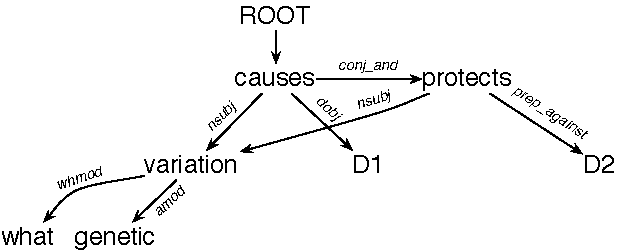
\includegraphics[width=0.48\textwidth]{stanford_parse}
&
\raisebox{2cm}{
\begin{tabular}{l}
cause (G?, D1) $\wedge$ % \\[0.5cm]
protect\_against (G?, D2)
\end{tabular}
}
\\
(a) step 1: syntactic parsing &
(b) step 2: semantic parsing\\[0.1cm]
\end{tabular}
\caption{Natural language parsing of the input query
{\em``What genetic variant causes D1 and protects against D2?"}
where D1 and D2 stand for two diseases.
(a) syntactic parsing: from query to Stanford dependencies.
(b) semantic parsing: from dependencies to first-order logic.
\label{fig:parse}}
\end{figure}
\vspace{-2ex}

The NLP step will result in a first-order logic formula (Fig.~\ref{fig:parse}(b)). This representation of the
user query will be used by the reasoning engine to generate a dossier of search
strategies.

%an identification of relevant abstract terms (such as ``disease,'' ``pathway,'', ``molecule'' etc.) along with a desired connectives between them (such as ``offers protection against,'' ``is associated to'' etc.).
\subsection{Generate a dossier of search strategies}
\label{section:strategies}
Given a parsed natural language query as input, our Reasoning Engine will return
a {\em dossier\/} of possible {\em search strategies.\/} A search
strategy is a {\color{red} graph} with vertices being biological entity types (including genetic
variants, drugs, genes, molecules, pathways, diseases, diagnoses,
etc.) and edges being query templates of Knowledge Sources to identify
relationships between pairs of those entities.
% Thus, each search strategy is a
%connected, undirected {\color{red} graph} in which each vertex corresponds to a type of
%biological entity and each edge corresponds to a Knowledge Source that can
%return associates between such entities.
%tuples of associations for the entity types corresponding to the respective vertices.
Terminal vertices in this {\color{red} graph} correspond to
the entity types of the constants provided by the user's parsed natural language
query. To illustrate, we show the {\color{red} graph} for three simple search strategies that
the reasoning engine would include in the dossier for two user queries: {\em How
  are disease DX and disease DY connected?\/} (Fig.~\ref{fig:ugraph}a-b) and
{\em How does variant G cause disease DX and protect against disease DY?\/}
(Fig.~\ref{fig:ugraph}c).
\begin{figure}[htbp]
%  \begin{tabular}{ccc}
  %%    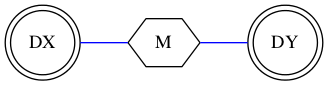
\includegraphics[width=1.2in]{net6.png} &
  \begin{center}
    \begin{overpic}[width=1.2in]{net6.png}
      \put (5,40) {{\large \textsf{\textbf{(a)}}}}
    \end{overpic} % &
    \begin{overpic}[width=2.2in]{net7.png} 
      %    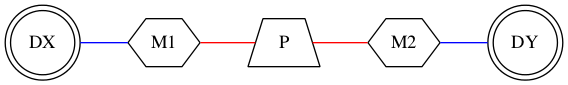
\includegraphics[width=2.2in]{net7.png} &
      \put (5,23) {{\large \textsf{\textbf{(b)}}}}
    \end{overpic}
    \begin{overpic}[width=2.5in]{net8.png}
      %    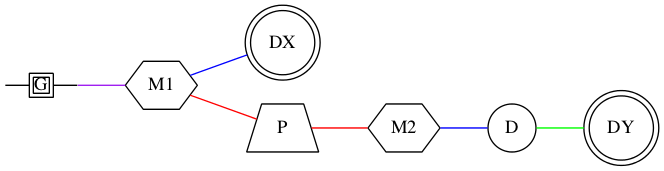
\includegraphics[width=2.5in]{net8.png} \\
      \put (5,20) {{\large \textsf{\textbf{(c)}}}}
    \end{overpic}
    \end{center}
%                    {\bf (a)} & {\bf (b)} & {\bf (c)}
 %                   \end{tabular}
  \caption{Three example search strategies returned by the reasoning engine: (a)
    and (b) are for a user query {\em How are disease DX and disease DY
      connected?\/} %, which has two constants.
        Search strategy (c) is for a
    query {\em How does variant G cause disease DX and protect against disease
      DY?}  Double-shapes denote constants in the query. Shapes denote bioentity
    type (circle: disease, hexagon: molecule, trapezoid: pathway, box:
    variant). Internal vertex labels like ``M'' and ``P'' representing the
    entity {\em type,} not a specific entity. Edge colors denote the type of
    association (blue: disease-molecule, red: molecule-pathway, green:
    disease-disease, purple: variant-molecule). 
    %Arbitrarily complex search
    %strategies can be created by chaining together additional possible
    %entity-entity relationships, however, our approach penalizes search strategy
    %graphs by the number of edges and strength of association, in order to prioritize simpler search
    %strategies.
    }
  \label{fig:ugraph}
\end{figure}
\vspace{-2ex}

\subsubsection{How the reasoning engine will generate and prioritize search
  strategies}

In implementing the reasoning engine, we will use a Markov chain approach to
generate undirected {\color{red} graphs} with the constant terms from the user's query as
terminal vertices in the {\color{red} graph}. This approach enables the prioritization of
search strategies with fewer Knowledge Source lookups.  To illustrate, recall the hypothetical user query {\em How are
  disease DX and disease DY connected?}. With two constants (i.e., terminal
vertices in the {\color{red} graph}), the reasoning engine would generate {\color{red} graphs} according to
the Markov process shown in Fig.~\ref{fig:mp}a).
\begin{figure}[h!]
  \begin{center}
  \begin{overpic}[width=2.5in]{markov1.png}
    \put (0,0) {{\large \textsf{\textbf{(a)}}}}
  \end{overpic}
  \begin{overpic}[width=2.5in]{markov2.png}
    \put (0,0) {{\large \textsf{\textbf{(b)}}}}
  \end{overpic}
  \end{center}
%  \begin{tabular}{cc}
%    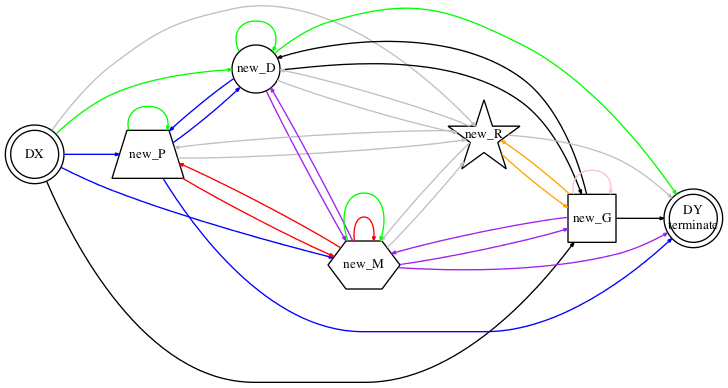
\includegraphics[width=3in]{markov1.png} %&
%    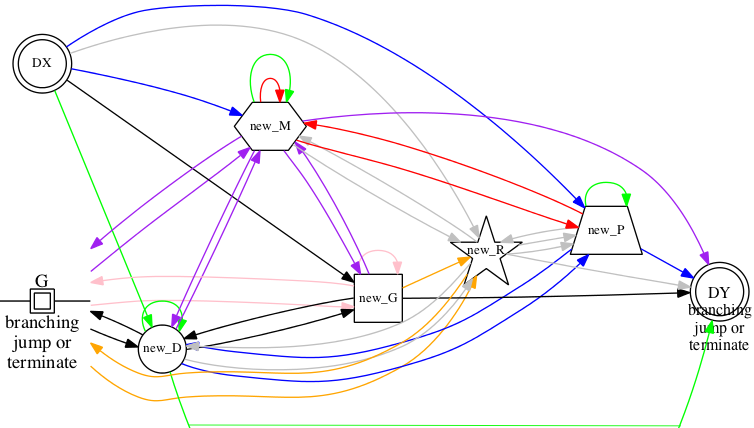
\includegraphics[width=3in]{markov2.png} %\\
%                    {\bf (a)} & {\bf (b)}
%  \end{tabular}
  \caption{Markov chain state transition graphs for generating ranked query strategies
    for (a) an example two-constant query (diseases DX and DY) and (b) a
    three-constant query (variant G and diseases DX and DY). Double-shape
    vertices are the constants of the natural-language query.  Colored arcs
    represent searches for entity-entity associations in various database
    sources [blue: disease-molecule association (e.g., DisGeNET, ClinVar), red:
      molecule-pathway association (e.g., Pathway Commons 2, BioCyc), green:
      disease-disease association (e..g, Monarch, DNetDB), purple:
      variant-molecule association (e.g., ClinVar, BeFree), pink:
      variant-variant association (SNAP or IGSR), orange: drug-variant
      interaction (PharmGKB), black: variant-disease association
      (ClinVar, DisGeNET)]. Each shape corresponds to a different type of
    biological entity (M: molecule, P: pathway, R: drug, G: variant, D:
    disease). In (b), the ``branching jump or terminate'' vertices enable the
    generation of a branched tree.}
%    state, the procedure is (i) add the indicated vertex to the undirected graph
%    being constructed, (ii) remove the indicated vertex from the transition
%    digraph, and (iii) select a non-leaf vertex in the undirected search
%    strategy graph and begin extending a branch from that vertex.}
  \label{fig:mp}    
\end{figure}
Such Markov chains will be constructed for each possible one-constant, two-constant,
and three-constant natural-language query (and are trivially extensible). 
%Markov chain edges will have a standard set of transition probabilities assigned.
 Each realization of the
Markov chain will generate a possible search strategy, i.e., an undirected {\color{red} graph},
%with the constant entities as terminal vertices; the Markov chain will also
and will assign a probability to each search strategy by penalizing weak associations and excessively long chains
of Knowledge Source lookups.
% and prioritizing the simplest strategies that can
%connect the constant entities.

\vspace{-2ex}
\subsubsection{Training of the Markov chain transition probabilities}
The transition probabilities (weights of the
colored edges in Fig.~\ref{fig:mp}) will be determined empirically using a set
of 100 natural-language queries that we will assemble from template queries from
online NCATS-Translator resources and using biological mechanisms (and
successful search strategies for these queries)
% that we will validate by hand)
for drug-variant interactions, variant-disease mechanisms, etc. We will select
transition probabilities that minimize the ranks of the 100~successful search
strategies for the 100 example queries, among the dossiers produced for these
queries (using the principal axes and eigenvalues of the Hessian to
prioritize important linear combinations of the log-probability weights to
be fine-tuned in the training pocedure).
\vspace{-2ex}
\subsubsection{A concrete example of how our reasoning engine would work}
Suppose a user wishes to find a common mechanism %to identify a common mechanism
underlying the causal effect of variant rs334 for sickle-cell anemia and that
same variant's protective benefit against malaria. The natural-language query
has three constants, %and one search strategy that would be ranked in the dossier would be the one shown in
and one possible search strategy is given in 
 Fig.~\ref{fig:ugraph}c. If executed against the
databases Pathway Commons (red), Disease Ontology (green), DisGeNET (blue), and
ClinVar (purple), the search strategy would return an explanatory mechanism, as
shown in Fig.~\ref{fig:malaria}, that is consistent with current knowledge of
the role of heme in cerebral malaria~\cite{Ferreira:2011ff}.
\begin{figure}[htbp]
  \begin{center}
    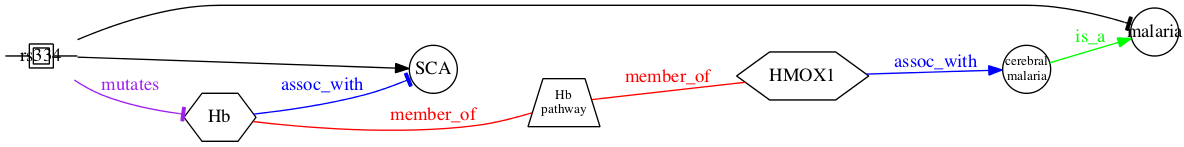
\includegraphics[width=6in]{net5.png}
  \end{center}
    \caption{Example of how the reasoning engine-returned search strategy of
      Fig.~\ref{fig:ugraph}c would find entity-entity associations that would
      suggest a common mechanism underlying the protective benefit of the rare
      variant rs334 against malaria and the causal effect of rs334 for
      sickle-cell anemia (SCA). Hb, hemoglobin b; HMOX1, heme
      oxygenase 1.  Edge colors: see Fig.~\ref{fig:mp}b.}
  \label{fig:malaria}
\end{figure}
\vspace{-2ex}


%% Knowledge Sources, specific queries against those knowledge sources that will
%% return tuples of entities , and join operations connecting those entities. If
%% we conceptualize these entities as Without loss of generality, we will denote
%% identify relevant knowledge sources and construct appropriate queries in
%% order to answer user questions. This is accomplished by constructing a
%% network of \textit{schemas} and other metadata of Knowledge Sources (KS's)
%% which we call a \textit{schema network}. This representation will not be a
%% network of all biological interactions and entities contained in the KS's,
%% but rather it compactly and abstractly represents the categories of
%% information contained in the various Translator KS's as well as the
%% relationships between them. Hence, nodes are metadata entities (such as
%% \verb|disease| or \verb|pathway|) and edges between them are given by first
%% order logical statements (such as \verb|assoc_with(X,Y)|). Using the parsed
%% user input, our Reasoning Engine will identify paths in this schema network
%% that represent search strategies to answer the user query. These paths will
%% traverse one or more KS's metadata and hence will automatically identify the
%% relevant databases to query. To find such paths, we will implement a
%% reasoning engine based on the formalism of Tractable First-Order
%% Probabilistic Logic and its associated Tractable Markov Logic (TML) language
%% developed by \citet{Domingos:2012wi}. The identification of such paths is
%% equivalent to knowledge-based model construction, which is known to be
%% subsumed by Markov Logic \cite{domingos20071}.


%\subsubsection{Tractable Markov Logic} In keeping with the distributed nature
%of Translator's Knowledge Sources, the reasoning engine that will generate the
%dossier will operate on a Markov Logic Network learned from the {\em schemas\/}
%and other metdata of Knowledge Sources; it will not be a network of all
%biological interactions contained in the Knowledge Sources. The reasoning
%engine's input will be a data structure representing the parsed natural
%language query (see Sec.~\ref{sec:nlp}). The reasoning engine's output will be
%a {\em dossier,\/} i.e., a ranked list of {\em search strategies,\/} where a
%search strategy is a possible joining of result-sets from one or more queries
%of Translator Knowledge Sources (KS).


%% The goal will be to find paths in the schema network that describe common
%% mechanisms between the input diseases. One possible kind of path is a
%% (disease,disease) tuple representing ``is a subtype of'' relationships
%% (Fig.~\ref{fig:networks}b). This kind of relationship between diseases is
%% inferred from the metadata of the Gene Ontology database. An alternate path
%% consists of a undirected edges $\{$disease,disease$\}$ representing
%% disease-disease associations from the DisGeNET database
%% (Fig.~\ref{fig:networks}c). A more complicated path (traversing two different
%% databases) is given in Fig.~\ref{fig:networks}b) where (molecule,disease)
%% ``associated\_with'' tuples (from DisGeNET or Pharos) with (molecule,pathway)
%% tuples representing ``member\_of'' relationships from Pathway Commons. An
%% example of a {\em three}-database search strategy, for the same user query
%% (Fig.~\ref{fig:threedb}a) about a variant-to-two-diseases association, is shown
%% in Fig.~\ref{fig:threedb}b).

\vspace{-2ex}
\subsection{Executing search strategies}
\label{section:Dijkstra}
After the search strategy ({\color{red} graph} generated by the Markov chain) is selected, we will
employ a modified Dijkstra algorithm to find paths between source and target
entities that minimize a sum of edge-weights, where smaller edge-weights
indicate stronger evidentiary value. The modification will ensure that, for
causal paths of influence, the overall ``sign'' of the path (activating or
inhibiting) is consistent with the semantics of the user's natural-language query.

%\subsubsection{Composition of the Markov Logic Network} We will use the
%Java-baesd (and open-source) NCATS-Tangerine Beacon Aggregator to obtain
%metadata (schemas and entity counts) from Knowledge Sources via RESTful queries
%leveraging the common Translator Knowledge Beacon Application Programming
%Interface (KBAPI).


%% Each of these possible paths identifies relevant KS's and represents a search
%% strategy: how to traverse these databases to answer the user query. A naive
%% approach to ranking these different search strategies would be to use a
%% combination of path length with edge weightings based on, say, prevalence of the
%% given diseases $D1$ and $D2$, strength of associations, etc. A more nuanced
%% approach is to utilize the TML language \citet{Domingos:2012wi} to rank the
%% search strategies in terms of how well they answer the user input. After the
%% user selects a desired search strategy (alternatively, the top ranked search
%% strategy is automatically utilized), the source and target nodes are grounded
%% with the particular biological entities contained in the user query. A modified
%% Dijkstra algorithm (Section \ref{section:Dijkstra}) is then used to execute the
%% query on the databases of interest to find paths between actual biological
%% entities.

%The schema network contains many different kinds of paths between a The schema
%network will contain various paths between the disease label and itself. For
%example, one such path is $D1$ ``is a``

%A simple strategy would be to search to obtain a list of (disease,disease)
%tuples representing ``is-a'' relationships from the Gene Ontology database
%(Fig.~\ref{fig:networks}b) where the edge would be assigned a weight in the
%Markov Logic Network based on the strength of evidence of this information type
%(either a fixed weight for the database, or with more information, the weight
%could be the ratio of prevalence of $D1$ to prevalence of $D2$). (We note that
%this search strategy would not be selected by the reasoning engine because the
%``is a'' relationship between two diseases is not consistent with the variant
%being protective against disease D2 and causal for disease D1). An alternative
%simple search strategy would be to load a list of {\em undirected\/}
%$\{$disease,disease$\}$ pairs representing disease-disease associations from
%the DisGeNET database (Fig.~\ref{fig:networks}c). An example of a {\em
%two}-database search strategy would be to join (molecule,disease)
%``associated\_with'' tuples (from DisGeNET or Pharos) with (molecule,pathway)
%tuples representing ``member\_of'' relationships from Pathway Commons
%(Fig.~\ref{fig:networks}d). An example of a {\em three}-database search
%strategy, for the same user query about a variant-to-two-diseases association
%(Fig.~\ref{fig:threedb}a), is shown in Fig.~\ref{fig:threedb}b.
%% \begin{figure}[h!]
%%   \begin{tabular}{ccc}
%%   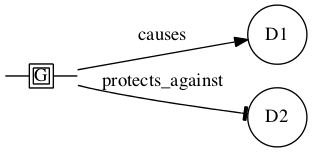
\includegraphics[width=1.4in]{baseproblem.png} &    
%%   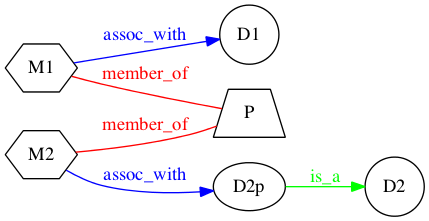
\includegraphics[width=2in]{net4.png} &
%%   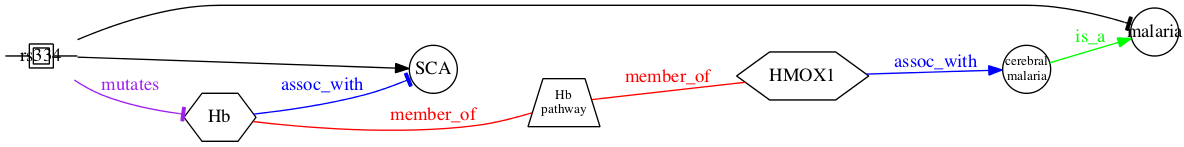
\includegraphics[width=2.5in]{net5.png} \\
%%                   {\bf (a) Query} & {\bf (b) Search Strategy 4} & {\bf (c) Search Result}
%%   \end{tabular}
%%   \caption{Example query predicate information (A); three-database example
%%     search strategy (B); matching search result for the specific query example
%%     G=rs334, D1=sicke-cell anemia (SCA) and D2=malaria (C). Edge color denotes
%%     the Knowledge Source to be searched (blue, DisGeNET; red, Pathway Commons;
%%     and green, Disease Ontology). Black edges denote the original query. Purple
%%     edge is the inferred interaction that explains the two black edges in light
%%     of the colored edges.}
%%   \label{fig:threedb}
%% \end{figure}
%% For example, assume that the variant G in this example query scenario is rs334,
%% a pleiotropic rare (MAF = 0.014\%) variant for which the homozygous minor allele
%% causes the blood disorder sickle-cell anemia (D1) and protects against malaria
%% (D2). A Dijkstra search on the three-database search strategy shown in
%% Fig.~\ref{fig:threedb}b) would yield a match indicating that a potential
%% explanation for the pleiotropy of rs334 is that it inhibits the hemoglobin
%% pathway, thus reducing circulating levels of free heme, which has been reported
%% to be protective in the case of cerebral malaria (a neurological complication of
%% malarial disease)~\cite{Ferreira:2011ff}.

\vspace{-2ex}
\subsection{Anticipated functionality for the POC reasoning tool}
%\textit{Functionality for the reasoning tool proof-of-concept (due in Nov)}
For the POC questions, the system we build will allow the user
to select from one of two questions: ``which genetic condition(s) protect(s)
from a given disease $D$'' and ``what is the outcome pathway for drug $D$ and
condition $C$''. The condition $C$ and/or drug $D$ will be
user-specified. Pre-computed search strategies for these two questions will be
implemented.  The modified Dijkstra algorithm will be implemented and will
search the Knowledge Sources in real time, based on the search query.  If funded, our full knowledge engine 
will allow for natural language input (Section
\ref{section:NLP}), automatic generation of search strategies (Section
\ref{section:strategies}) and will account for empirically determined
evidentiary weights for different types of entity-entity associations
(Sec.~\ref{section:Dijkstra}).%also utilize the Dijkstra algorithm of
%Section \ref{section:Dijkstra}.

\vspace{-2ex}
\subsection{Components of the proposed software stack}
We will implement our system in Python, using \verb|graph-tool| \cite{peixoto_graph-tool_2014} or \verb|SNAP| \cite{leskovec2016snap} for
graph searching and querying, \verb|Boost.Python| \cite{boostpython} for implementing the
modified Dijkstra algorithm, \verb|Py4J| \cite{Py4J} for accessing Java-only
APIs as needed (see Sec.~\ref{sec:interact}), \verb|Flask| \cite{grinberg2014flask} for providing a REST
API, and \verb|Requests| and the standard library \verb|json| to access the REST API for the NCATS
blackboard. We will use a Python API for Stanford CoreNLP \cite{manning2014stanford}.  We will publish on GitHub all
code developed with NCATS support.

%% The natural language processing will use the open source software \textbf{Liang:
%%   name and reference}. {\color{red} For the search strategy generation, there
%%   are a number of open source software packages that implement Markov Logic
%%   Networks: Tuffy \cite{DBLP:journals/pvldb/NiuRDS11}, Alchemy
%%   \cite{kok2006alchemy}, RockIt \cite{noessner2013rockit}, and TheBeast
%%   \cite{riedel08improving}.}


%\subsubsection{Natural language query analyzer} \label{sec:nlp} Should we use
%the Stanford CoreNLP with BioNLP shared task data? If so, which Python API
%should we use? (There are about a dozen of them).

\vspace{-2ex}
\subsection{How proposed software will interact with Translator}
\label{sec:interact}
We will use the Java-based NCATS Knowledge Beacon Aggregator to obtain metadata
(i.e., schemas and entity counts) from Knowledge Sources via RESTful queries
leveraging the common Translator Knowledge Beacon Application Programming
Interface (KBAPI). Our system will provide the functionality of converting a
natural-language-query to a dossier of search strategies, via a REST API
complying with the NCATS Knowledge Beacon Web API. Results will be served in JSON form, formatted by a web interface.

\vspace{-2ex}
\subsection{Beyond Markov chains---Markov Logic Networks}
We would additionally investigate the potential utility for constructing a
Markov Logic Network~\cite{Domingos:2012wi,domingos20071} that would
probabilistically represent possible connections between different types of
biological entities in different Knowledge Sources, as well as the nature of
those connections (e.g., inhibitory, causal, etc.). Such a model would represent
a generalization of the undirected graphical models that constitute the superset
of search strategies in our first reasoning engine prototype. As such, the use
of Markov Logic Networks could improve the ability to map parsed
natural-language queries to the search strategies that are most likely to yield
biologically relevant information.


%% \section{Background: Types of questions} \subsection{How does drug X induce
%% clinical outcome Y?}  \subsection{Why do variants that cause sicke-cell
%% anemia protect against malaria?}  \subsection{In people with variants found
%% in any of the 22 known FA genes, is there increasing incidence of apalastic
%% anemia (or other diseases)?}  \subsection{What venomous species have resulted
%% in drugs approved by the FDA?}  \subsection{What cellular processes in which
%% tissues are impacted in a patient-based EMR?}  \subsection{Why does ingestion
%% of GlcNAc ameliorate symptoms of ngly1 deficiency?}

%% \section{Background: Knowledge Sources}
%% \begin{description}
%% \item[EBI String]{Protein-protein interactions}
%% \end{description}

%\section{Personnel}

\bibliographystyle{plainnat}
\bibliography{conclett}

\end{document}
